\documentclass[tikz,border=10pt]{standalone}
\usepackage{tikz}

\begin{document}

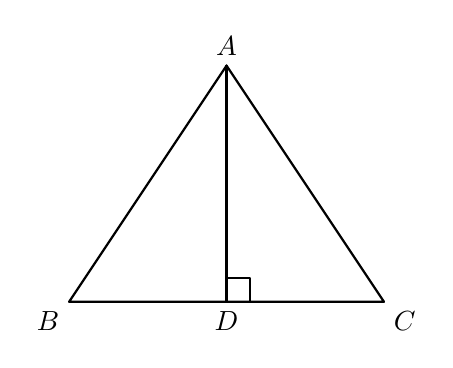
\begin{tikzpicture}[scale=1, line cap=round, line join=round]

% --- Coordinates ---
\coordinate (A) at (0,3);
\coordinate (B) at (-2,0);
\coordinate (C) at (2,0);
\coordinate (D) at (0,0);

% --- Drawing ---
% Draw the main triangle ABC
\draw[thick] (A) -- (B) -- (C) -- cycle;

% Draw the altitude AD
\draw[thick] (A) -- (D);

% Draw the right-angle symbol at D
\draw[thick] (0,0.3) -- (0.3,0.3) -- (0.3,0);

% --- Labels ---
\node[above] at (A) {$A$};
\node[below left] at (B) {$B$};
\node[below] at (D) {$D$};
\node[below right] at (C) {$C$};

\end{tikzpicture}

\end{document}
